%-----------------------------------------------------------------------------------%
\section{Introduction\label{sec:intro2dm}}
%-----------------------------------------------------------------------------------%

tell a story about dark matter in a nutshell.

Dark Matter (DM) has been a whispering problem in physics for almost 100 years.
Anomolies have been detected by way of weird galaxy behaviour, budding Cosmology, and more \ns.
It was sometime in 1930's when the super duper smart Zwicky measured that it was defintely there.
It's kind of a big deal because we have no idea what the nature of this stuff and there's a lot of it.
According to Lambda CDM, the most legit model, \ns DM is about 85\% \fu, of all mass in the universe.
It's called dark in fact because we cannot see it. \ns
Finding out what the hell it is, is an active field of research and hopefully it interacts with the standard model.

Here's what we do know about DM so far\dots
DM is dark, it doesn't interact readily with light.
DM also doesn't interact noticably with the other standard model forces (EM, Strong, Weak) at a rate that matters \ns.
DM is cold.
By cold I mean that it is most likely not moving at relativisic speeds like neutrinos and photons. \ns
If it was moving that fast, the structures we see like galaxies would be much more diffuse than what is observed. \ns
DM is old.
DM played a critical role in the formation of the universe and the structure within it. \ns
We know this from Cosmology and computer universe simulations \ns.

The search for DM is basically summarized by trying a bunch of different models and performing measurements of all kinds to test them.
These models of course have to nominally agree with the known observations seen over the last century.
Whenever we perform a test and don't see anything, the parameter spaces gets more contrained.
I discuss some of the ideas ad approaches further on.
I Especially discuss the models that are relavent to my thesis.

We forunately have the largest volume and lifetime ever for a particle physics experiment in the universe.
This means we can do some pretty cool shit very efficiently.
The drawn back are the backgrounds.

My these is organized like the following.
\todo
\color{purple}Text should look like ...
Chaper x has blah blah blah.
\color{black}

%-----------------------------------------------------------------------------------%
\section{Evidence for Dark Matter\label{sec:evidence4dm}}
%-----------------------------------------------------------------------------------%

Let me show you why we're pretty sure DM is a thing and why it might be particle like in nature.
My thesis focuses on WIMP dark matter which is one of the better motivated things out there
There were some weird as fuck anomolies early in the last century but we weren't 100\% that it was legit.
Then some great scientsist made some keen measurements of stars and their minds were blown.
Read more to see what we know now.
I promise you're about to get mind fucked.

%$$$$$$$$$$$$$$$$$$$$$$$$$$$$$$$$$$$$$$$$$$$$$$$$$$$$$$$$$$$$$$$$$$$$$$$$$$$$$$$$$$$%
\subsection{First Clues: Stellar Velocities\label{sec:ev4dm_stars}}
%$$$$$$$$$$$$$$$$$$$$$$$$$$$$$$$$$$$$$$$$$$$$$$$$$$$$$$$$$$$$$$$$$$$$$$$$$$$$$$$$$$$%
Ok so someone \fu \ns started taking measurments with at.
They were curious about what speed stars were orbitting the galaxies they were contained in.
These measurements were done for things close by.
At the time we were even that sure galaxies were a thing.
Bu with the basical knowlwedge we had we used the virial theorem with the velocities of the stars to measure the mass inderectly of the galaxies.

\emptyeq{The Virial Eqn}

\todo{explain the virial equation}
\ns you probably want to source the theory behind why this important

The verdict wasnt clear however until Vera Rubin made some awesome discoveries with more precise equipment and 21cm lines of Hydrogren gas in the galaxies.
This really showed that there was some unexplained discrepancy between how much mass we were seeing in the stars and the mass measured indirectly.
The issue is that it we're pretty sure now that we're not just under-estimating the mass of the stars \ns.
The difference in mass was up to 5x which is way way too much for what our uncertainties were (somewhere around 20\%)\ns.

\todo insert a velocity dispersion FIGURE here.
\ns the figure will need a source.

Nowadays we have more measurements of the stellar velocities and have even discovered small DM dense bodies called dwarf spheroidals (dSph)
These measurements have been made by the community \fu and there are compiled lists of how much DM these objects have.
Most of these measurements are made from newtonian virial theorem measurments.
There has since emerged new evidence.
These innovative techs are discussed in the following sections. The evidence cullminates into a story of particle dark matter.

%$$$$$$$$$$$$$$$$$$$$$$$$$$$$$$$$$$$$$$$$$$$$$$$$$$$$$$$$$$$$$$$$$$$$$$$$$$$$$$$$$$$%
\subsection{Mounting Evidence for Dark Matter\label{secc:ev4dm_more}}
%$$$$$$$$$$$$$$$$$$$$$$$$$$$$$$$$$$$$$$$$$$$$$$$$$$$$$$$$$$$$$$$$$$$$$$$$$$$$$$$$$$$%
Modern evidence for dark matter comes from new avenues.
We got microlensing which supports DM in the general relativity sector.
The Cosmic Microwave Background shows that the universe has DM in it from a very early stage.
The CMB is the primordial light from the young universe.
Basically a baby photo.
Then we have computational models where we model the universe.
Then we look at how the simulated universes look like compared to what we see.
From those simulations we infer how much dark matter is in the universe.
The fuller explinations and shortcoming of each of these methods is explained further in this section.

someone took a an observation of the bullet cluster.
The microlensing of galaxy clusters are some of the most damning evidence that DM is actually matter and not just a flaw in our gravitational theories.
There were two galaxy clusters \fu.
They clearly passed through each other at some point in the past and are in the process of merging \ns.
Two observations of the clusters were made independantly of each other.
The first was the microlensing of light around the galaxies due to their gravitational influences.
When celestial bodies are large enough, the gravity they exert bends space and time itself.
This bending effects light and will deflect light in a smilar way to how lenses will bend light.

\todo insert gravitational lensing figure compared to glass lensing. \ns.

With a sufficient understanding of light sources behind a celestial body, you can reconstruct the countours of the gravitational lenses.
The gradient of the contours then tells you how dense the matter is and where it is.

They then made measurements of the x-ray emmision from the clusters.
The idea is that since these galaxies are mostly gass and are merging, then they should be getting hotter.
If they're merging, the x-ray emmisions should be the strongest where the gas is mostly moving through each other.
The x-rays basically map out where the gas is in these merging galaxies.

\todo insert bullet cluster photo. \ns.

The dope super interesting thing is that the map of the x-ray emmisions totally doesnt align with the gravitational countours from the microlensing.
This incongruence is really telling that there is a lot of matter somewhere that we jsut cannot see.
Moreover this matter is NOT BARYONIC.
So then what is it?
This measurement didn't really tell us what exactly, but it did suggest that this DM also doesn't interact with itself very strongly.
If it did, then it would have been more aligned with where the x-ray emmision was.
There's been other studies of galaxies with similar results altho there are a handful that resemble something we expect for strongly self-interacting DM. \ns.
This result really makes it hard to argue that DM is somehow something amiss in our gravitational theories.

we got the CMB and geometry of the universe.
So there's this thing called the cosmic Microwave Background (CMB).
It's the universes baby photo from when all of the hydrogen de-ionized to form atoms.
This happened cause it was cold enough finally from the expansion of the universe.
The recombination happened someitme around less than 1 mil years after the universe was born \fu \ns.
when hydrogen absorbs an electron, it releases a photon of a specific wavelength.
This wavelength amounts to 13 ev or so according to the qm eqn\dots

\todo insert hydrogen energy level equation

However the universe has been expnding since it's creation.
In fact the time and space itself is exanding away from us for as long as the universe is old.
This red-shifts the combination light into the Microwave frequencies.
This is the light we can detect with microwave observatories and is what was first detected by so and so in the 19?? \ns \fu
This make a microwave image seen below after we subtract the average of the image.

\begin{figure}[h]
\centering{
    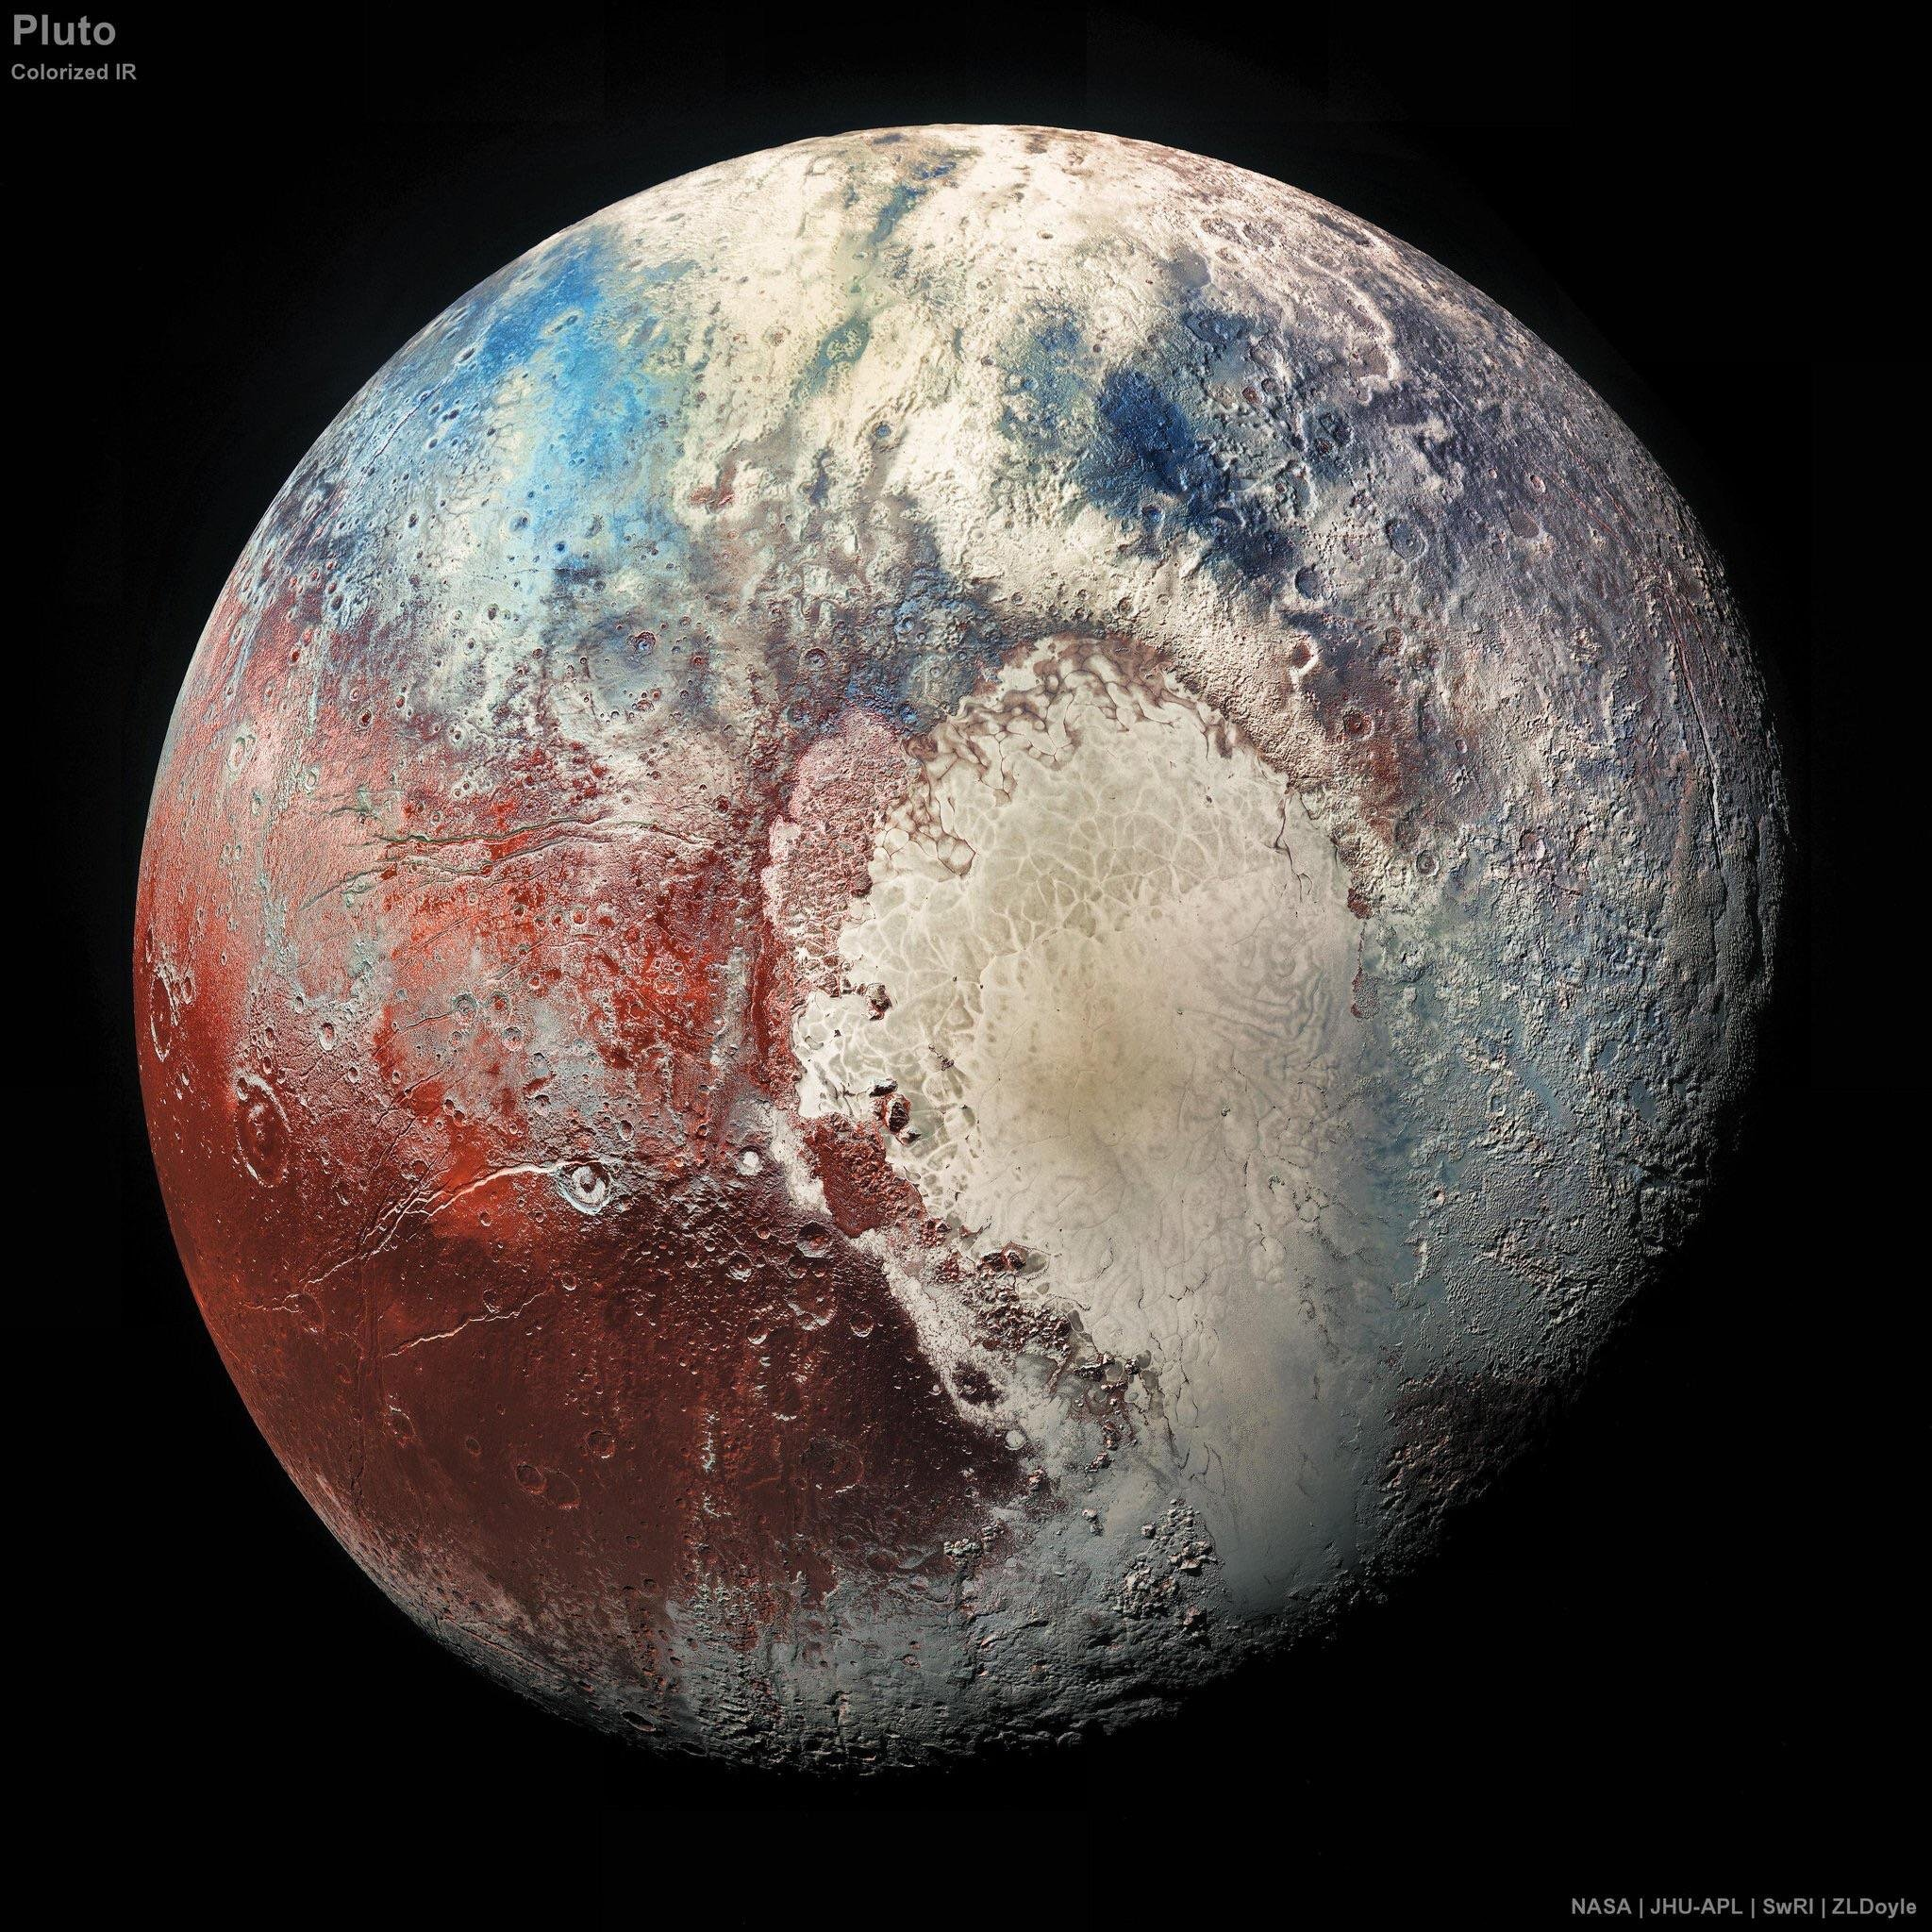
\includegraphics[scale=0.15]{figures/prettypluto.jpg}
    \caption{\\todo CMB PHOTO \ns \fu}
}
\end{figure}


We can do a funny thing with the photo but it's fairly straight forward.
Shove the photo into a spherical harmonic decomposition.
This gives you the vibrational modes of the CMB and therefore the early universe.
The important thing to note is that the harmoincs are based on primordial baryonic acoustic oscillations \fu
This is directly linked with the energy density of the universe and how these couple.
It's a cosmology and geometry thing.

\begin{figure}[h]
\centering{
    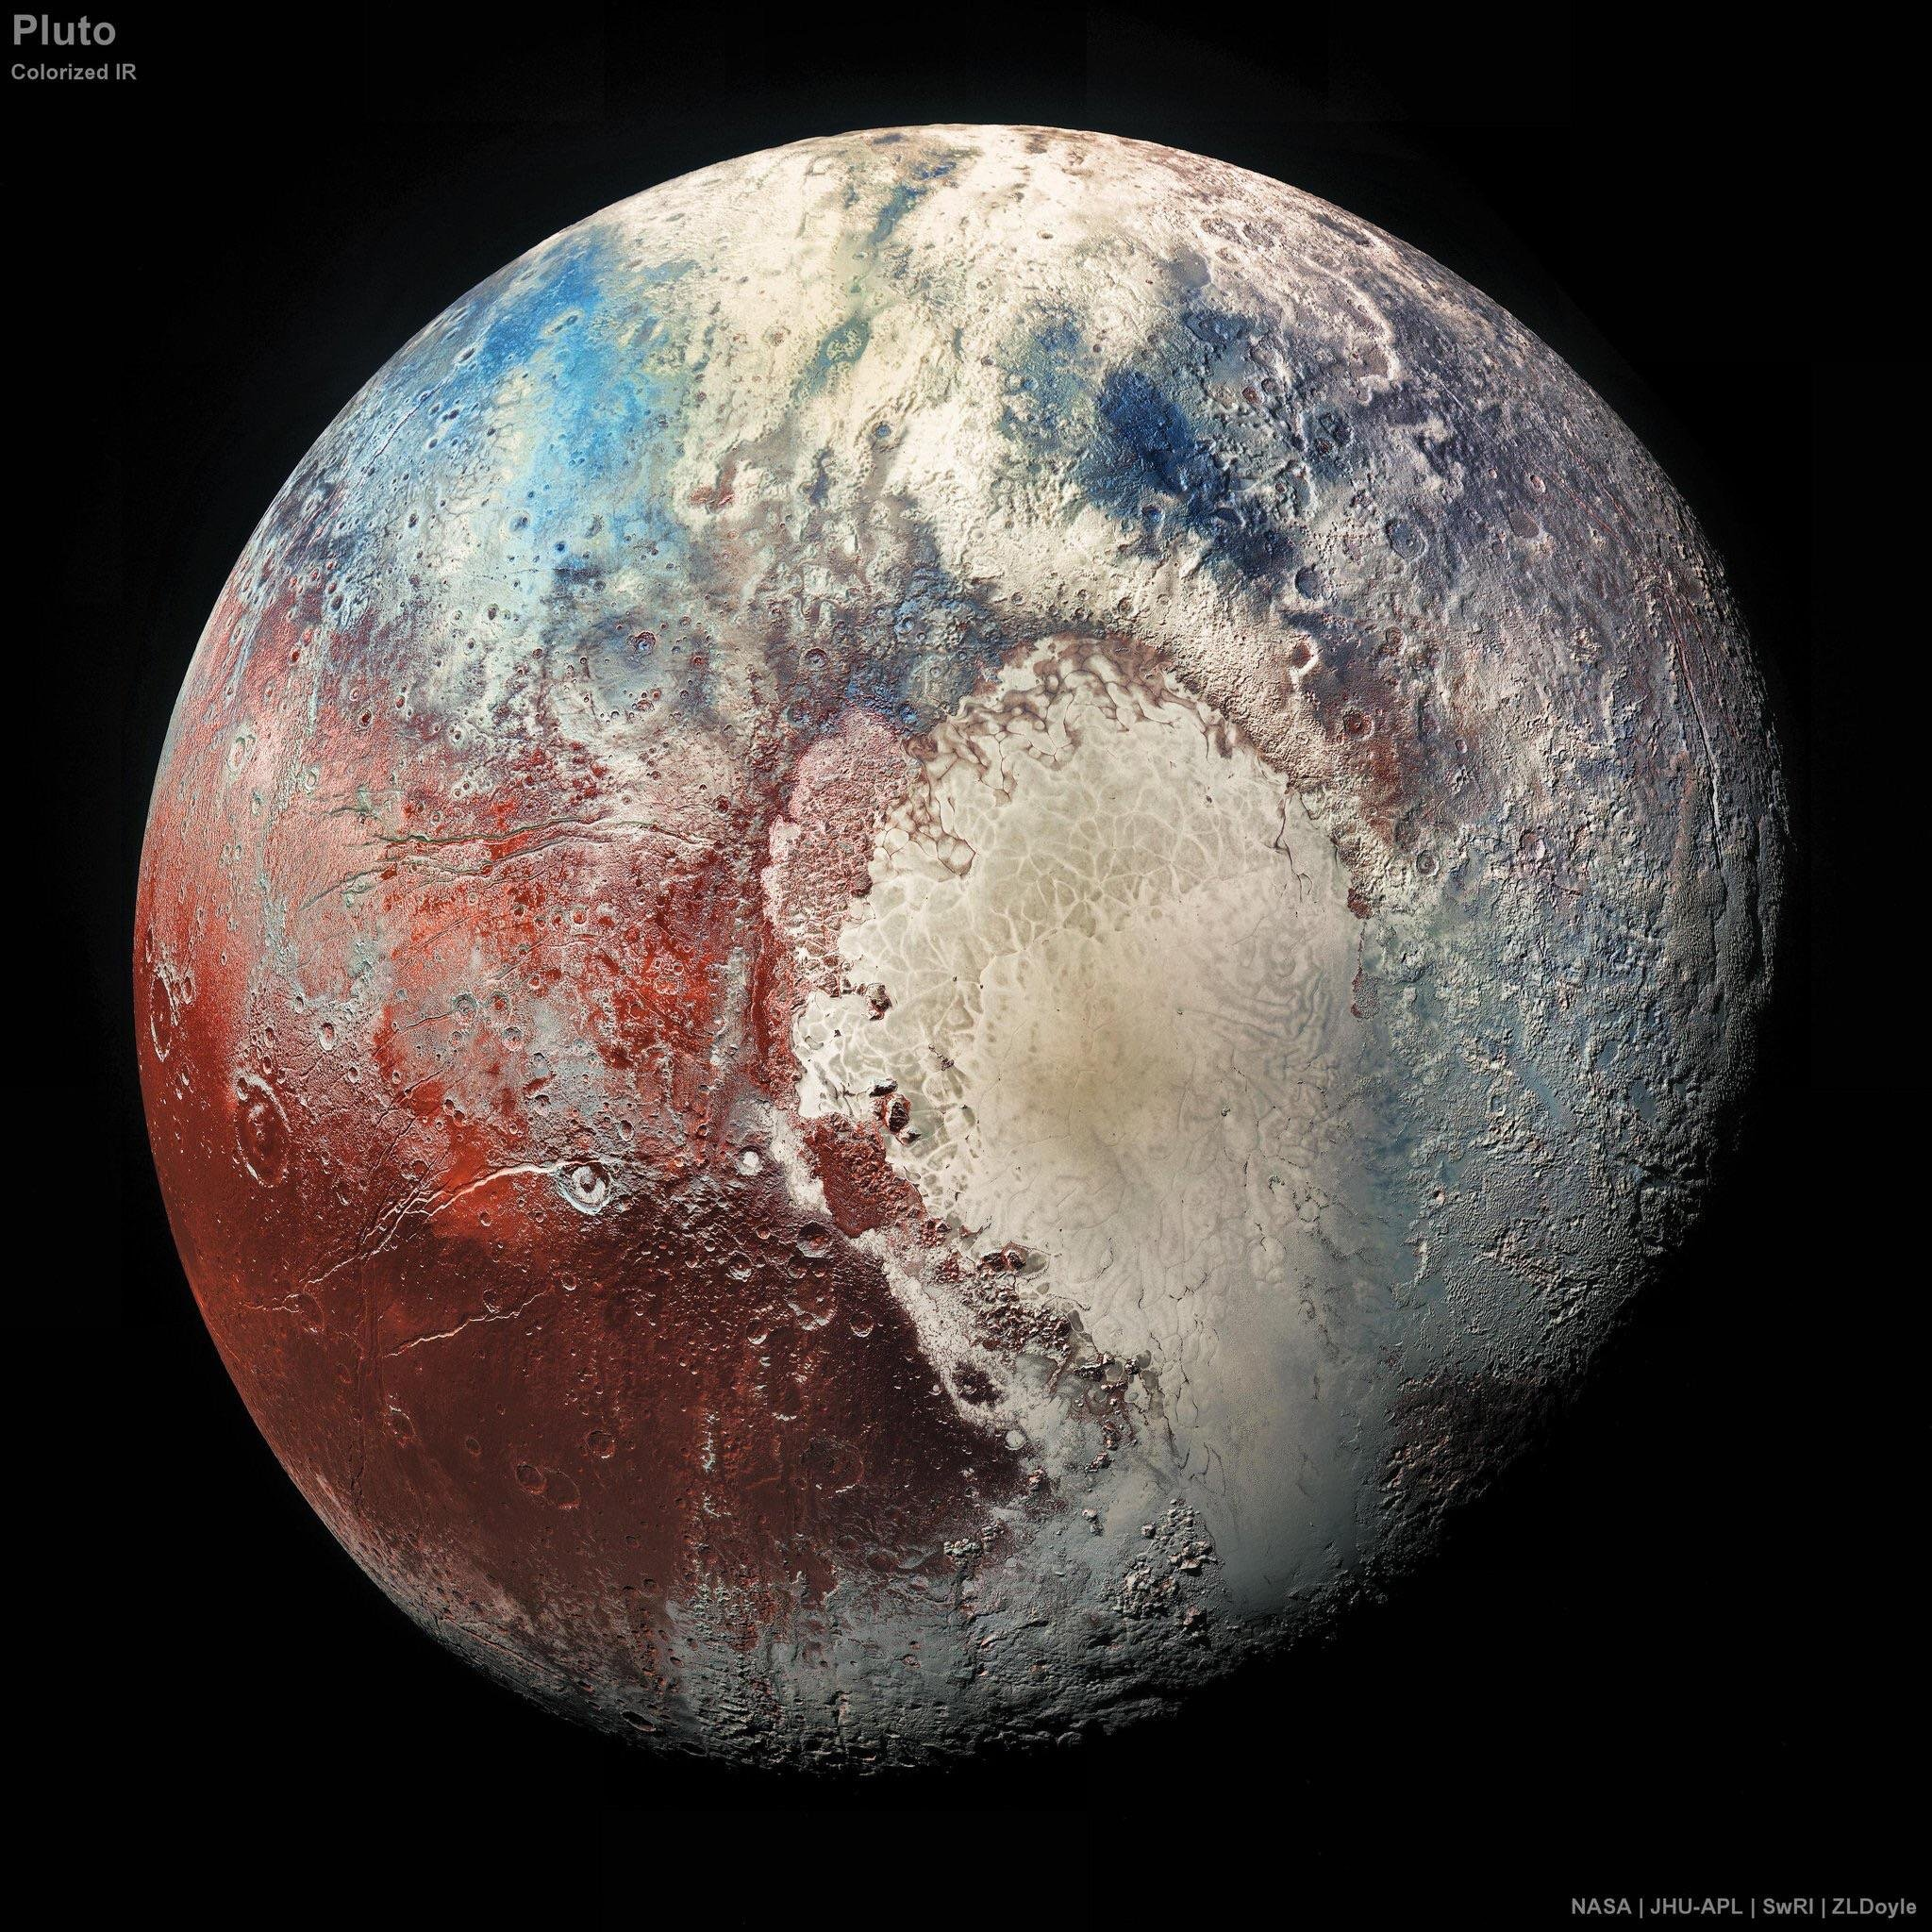
\includegraphics[scale=0.15]{figures/prettypluto.jpg}
    \caption{\todo FIGURE show plank harmoincs.}
}
\end{figure}

The harmnics would look very different for a universe with less dmm (see fig bla) or a lot more dm (see fig bla)

\todo show different harmonic oscillation diagrams.

The observations fit well with the Lambda CDM model and we derive the primordial dm concentration to be XX\% and primordial DM to be XX\%.
\todo What are the shortcomings? I think the most obcious arguement is simply that this is very old light, up to 13.6 billion years old.
It's not at all necessary that the universe shares the exact same DM, matter ratio.
There is a poorness in fit in the lower region of the graph and this is unexplained.
The way we measure distance can be really fucked sometimes so maybe that's a problem too.

Finally we have universe simulations like the millenium simultation and more \fu \ns.
These are computer simulations of the unverse with different fractions of DM and baryonic matters.
Additionaly hypotheses are tested like how hot the DM is and how strongly it interacts with itself and with baryonic matter.
These simulations are also done for smaller scales like galactic formation and galaxy clustering.
In alls cases the simulations most resemble out universe for a Lambda CDM like universe.

The main issues with the similations is mostly that we cant perfectly simulate the unverse.
They are often imcomplete with how they treat baryonic matter and make big assumptions about dark matter.
These simulations also have to contend with very real computational limitations.
The resultion of some of the universe simulations are as large at XX's of solar masses.
There's reason to beleive that the resultion might really matter as well. \ns \fu


Overall this forms a compelling arguement for dark matter.
However, these observations really only confirm that DM is there.
It takes another leap of theory to make observations of DM that are nongravitational.
One of which is the emergence of the Weakly Interacting Massive Particle hypothesis of DM.
This DM candidate theory is discussed futher in the next section.


SPACE TIME CURVY

%-----------------------------------------------------------------------------------%
\section{The WIMP Miracle\label{sec:dm_wimps}}
%-----------------------------------------------------------------------------------%

%-----------------------------------------------------------------------------------%
\section{Searching for Dark Matter\label{dm_search}}
%-----------------------------------------------------------------------------------%

%$$$$$$$$$$$$$$$$$$$$$$$$$$$$$$$$$$$$$$$$$$$$$$$$$$$$$$$$$$$$$$$$$$$$$$$$$$$$$$$$$$$%
\subsection{Shake it, Break it, Make it\label{sec:bop_it}}
%$$$$$$$$$$$$$$$$$$$$$$$$$$$$$$$$$$$$$$$$$$$$$$$$$$$$$$$$$$$$$$$$$$$$$$$$$$$$$$$$$$$%

%$$$$$$$$$$$$$$$$$$$$$$$$$$$$$$$$$$$$$$$$$$$$$$$$$$$$$$$$$$$$$$$$$$$$$$$$$$$$$$$$$$$%
\subsection{Break it: Standard Model Signatures of Annihilating Dark Matter\label{sec:break_it}}
%$$$$$$$$$$$$$$$$$$$$$$$$$$$$$$$$$$$$$$$$$$$$$$$$$$$$$$$$$$$$$$$$$$$$$$$$$$$$$$$$$$$%

%-----------------------------------------------------------------------------------%
\section{Multi-Messenger Dark Matter}
%-----------------------------------------------------------------------------------%

%-----------------------------------------------------------------------------------%
\section{Search Targets for Dark Matter\label{sec:dm_targets}}
%-----------------------------------------------------------------------------------%

%$$$$$$$$$$$$$$$$$$$$$$$$$$$$$$$$$$$$$$$$$$$$$$$$$$$$$$$$$$$$$$$$$$$$$$$$$$$$$$$$$$$%
\subsection{Dwarf Spheroidal Galaxies\label{sec:dSphs}}
%$$$$$$$$$$$$$$$$$$$$$$$$$$$$$$$$$$$$$$$$$$$$$$$$$$$$$$$$$$$$$$$$$$$$$$$$$$$$$$$$$$$%